\chapter{Đối ngẫu Fourier, động lượng và chuyển động của hạt tự do}

\section{Từ nền tảng đến ví dụ}

Sự vướng víu nằm ở trung tâm của cơ học lượng tử, nhưng các nền tảng nay đã được trình bày đủ rõ để ta có thể bắt đầu vận dụng chúng. Cho đến nay, học phần này dựa vào những hệ được cố ý chọn là nhỏ: một spin, một thiết bị có thể xoay, một danh sách hữu hạn các kết quả, và các phép đo lặp lại để từ đó suy ra xác suất. Những thí nghiệm ấy đơn giản hơn về mặt logic so với con đường lịch sử dẫn tới sự phát hiện cơ học lượng tử, nhưng chúng chứa các thành phần thao tác tối thiểu.

\begin{classroomqa}
\audiencequestion{Trong cơ học lượng tử, điều gì đóng vai trò tương tự tập nhỏ các điểm xuất phát thực nghiệm của Newton?}
\lecturerresponse{Một mô hình tối thiểu là thiết bị đo spin có thể xoay. Chuẩn bị một spin, chọn một trục, nhấn nút đo, ghi lại \(+1\) hoặc \(-1\), rồi lặp lại thí nghiệm cho đến khi biết các tần suất kết quả. Không gian vectơ, các đại lượng quan sát, các biên độ và quy tắc Born tổ chức các thống kê ấy. Về mặt lịch sử, lý thuyết xuất hiện từ một tập hợp hiện tượng nguyên tử phong phú hơn nhiều, nhưng về mặt logic thí nghiệm hai kết quả này là đủ để bộc lộ cấu trúc của nó.}
\end{classroomqa}

\begin{classroomqa}
\audiencequestion{Có phải cùng một quy trình thống kê phải được thực hiện cho từng đại lượng vật lý, chẳng hạn spin hay động lượng không?}
\lecturerresponse{Đúng. Một đại lượng quan sát gắn với một lớp cách bố trí thí nghiệm và các kết quả có thể có. Hình thức luận dự đoán phân bố một khi trạng thái và đại lượng quan sát đã được chỉ rõ, nhưng ý nghĩa vật lý của đại lượng ấy được xác định bởi cách nó được đo.}
\end{classroomqa}

Trước khi rời khỏi chủ đề vướng víu, có một câu hỏi từ phần thảo luận trước đáng được trả lời đầy đủ. Hãy xét hai electron với các sector singlet và triplet, và đưa trường bức xạ vào như một phân hệ lượng tử khác. Trường bức xạ có trạng thái chân không \(\ket{0_\gamma}\) và trạng thái một photon \(\ket{1_\gamma}\). Bản thân số hạt cũng có thể ở trạng thái chồng chập; không có quy tắc nào giới hạn sự chồng chập chỉ vào các trạng thái khác nhau của một số hạt cố định.

Đối với chuyển tiếp lý tưởng hóa được thảo luận trên lớp, một trạng thái electron ban đầu không vướng víu có thể được viết thành chồng chập của các thành phần singlet và triplet,
\begin{equation}
\ket{\uparrow\downarrow}
=
\frac{1}{\sqrt{2}}
\left(\ket{S}+\ket{T_0}\right).
\end{equation}
Ban đầu không có photon hiện diện, nên trạng thái là
\begin{equation}
\ket{\Psi(0)}
=
\frac{1}{\sqrt{2}}
\left(\ket{S}+\ket{T_0}\right)
\otimes\ket{0_\gamma}.
\label{eq:l9-initial-radiative-state}
\end{equation}
Thành phần singlet vẫn là singlet mà không phát xạ, còn thành phần triplet kích thích có thể thư giãn về singlet và phát ra một photon:
\begin{align}
\ket{S}\ket{0_\gamma}
&\longrightarrow
\ket{S}\ket{0_\gamma}, \\
\ket{T_0}\ket{0_\gamma}
&\longrightarrow
\ket{S}\ket{1_\gamma}.
\end{align}
Tính tuyến tính khi đó cho
\begin{equation}
\ket{\Psi_{\mathrm{final}}}
=
\ket{S}\otimes
\frac{\ket{0_\gamma}+\ket{1_\gamma}}{\sqrt{2}}.
\label{eq:l9-final-radiative-state}
\end{equation}

\begin{figure}[htbp]
\centering
\includegraphics[width=0.88\textwidth]{lecture_09_figure_01.png}
\caption{Trạng thái electron được phân rã thành các thành phần singlet và triplet rồi lấy tích tensor với chân không photon trước khi thư giãn bức xạ.}
\lectureframe{00:05:10}
\end{figure}

Biểu thức cuối cùng là một tích tensor giữa cặp electron và trường bức xạ. Hai electron vướng víu với nhau vì \(\ket{S}\) là trạng thái vướng víu, còn trường bức xạ được để lại trong trạng thái chồng chập của không photon và một photon. Ví dụ này tinh tế vì tương tác đã phân bố lại sự vướng víu: trạng thái tích ban đầu của các electron tiến hóa thành một cặp electron vướng víu, nhưng trạng thái electron–bức xạ lý tưởng hóa cuối cùng lại phân tích thành tích.

\begin{classroomqa}
\audiencequestion{Liệu bất kỳ photon tới nào cũng có thể đảo ngược chuyển tiếp và làm hai electron hết vướng víu không?}
\lecturerresponse{Không. Quá trình đảo thời gian đòi hỏi trạng thái photon, mode, pha, năng lượng và lịch sử tương tác thích hợp. Việc phản xạ photon đã phát trở lại chỉ là cách nói tắt cho việc sắp đặt sự tiến hóa nghịch đảo của toàn bộ hệ kín, chứ không phải khẳng định rằng một photon tùy ý sẽ xóa bỏ sự vướng víu.}
\end{classroomqa}

\begin{classroomqa}
\audiencequestion{Điều gì khiến triplet phát xạ nếu không đưa vào từ trường ngoài nào?}
\lecturerresponse{Các electron tương tác với nhau và với trường điện từ lượng tử hóa. Tương tác phụ thuộc spin của chúng làm cho một cấu hình spin thuận lợi hơn về năng lượng, và phần năng lượng dư có thể thoát ra dưới dạng bức xạ. Không cần một thiết bị đo bên ngoài nào; đây là động lực học đơn nhất thông thường của hệ kết hợp gồm các electron và trường.}
\end{classroomqa}

Sau khi giải quyết xong điểm còn lại đó, giờ ta gác spin sang một bên và nghiên cứu bài toán chuyển động đơn giản nhất: một hạt trên một đường thẳng một chiều.

\section{Sóng phẳng và cặp Fourier}

Trước khi quay lại vật lý, ta cần một đoạn xen vào về toán học. Bắt đầu với
\begin{equation}
e^{ipx}=\cos(px)+i\sin(px).
\end{equation}
Ở giai đoạn này, \(p\) chỉ đơn giản là một số thực điều khiển tốc độ dao động. Biểu thức này không phụ thuộc thời gian và vì thế chưa mô tả một sóng đang chuyển động. Nó được gọi là sóng phẳng vì, khi là một hàm của \(x\), nó có dạng hình sin quen thuộc.

Một lớp rộng các hàm đủ chính quy có thể được phân rã thành các mode như vậy. Ta giới hạn sự chú ý vào những hàm cư xử đủ tốt để các tích phân bên dưới có nghĩa: chúng không được phép bùng lên ở vô cực không gian, và về sau các hàm sóng vật lý sẽ khả tích bình phương. Với một quy ước chuẩn hóa đối xứng, cặp Fourier là
\begin{align}
\psi(x)
&=
\int_{-\infty}^{\infty}
\frac{dp}{\sqrt{2\pi}}\,
\widetilde{\psi}(p)e^{ipx},
\label{eq:l9-fourier-forward}\\
\widetilde{\psi}(p)
&=
\int_{-\infty}^{\infty}
\frac{dx}{\sqrt{2\pi}}\,
\psi(x)e^{-ipx}.
\label{eq:l9-fourier-inverse}
\end{align}
Hệ số \(\widetilde{\psi}(p)\) là biên độ phức của mode mang nhãn Fourier \(p\). Các thừa số \(1/\sqrt{2\pi}\) là theo quy ước; đặt một thừa số trong mỗi phép biến đổi làm cho hai công thức trông đối ngẫu với nhau. Dấu trừ tương đối trong số mũ là thiết yếu.

\begin{figure}[htbp]
\centering
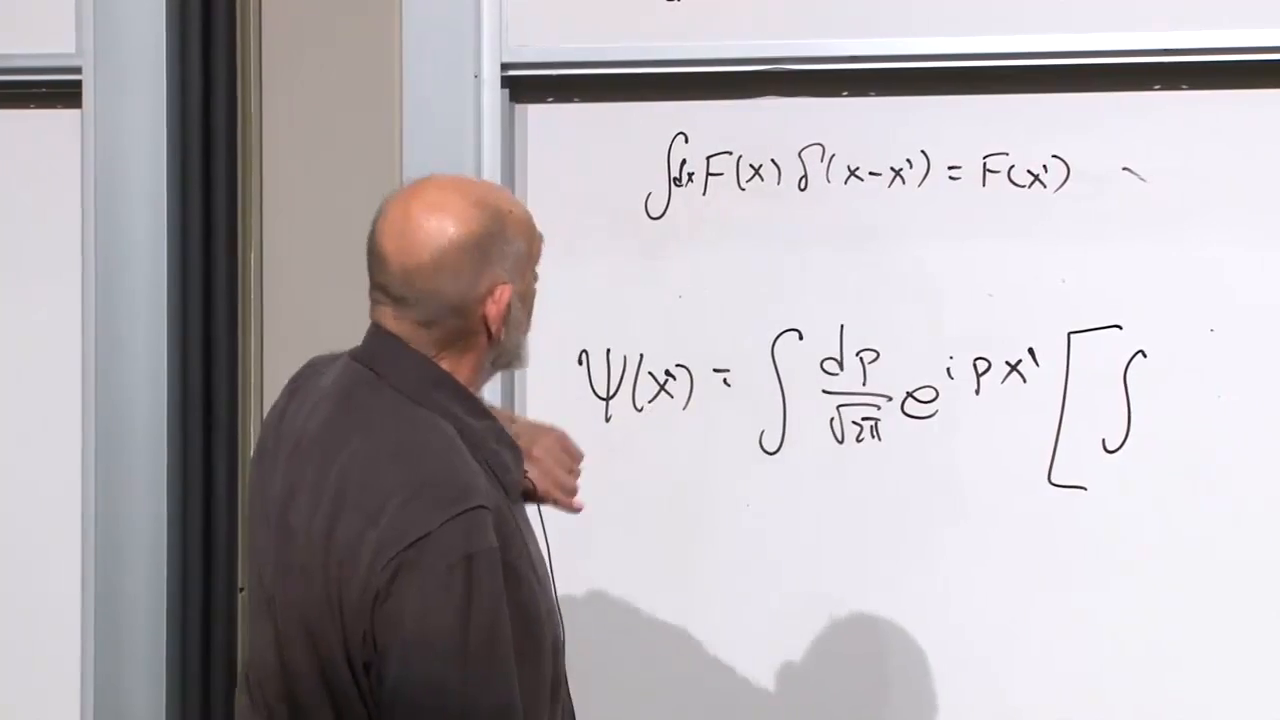
\includegraphics[width=0.88\textwidth]{lecture_09_figure_02.png}
\caption{Cặp Fourier đối xứng: một hàm được phân rã thành các sóng phẳng, và các biên độ mode được khôi phục bằng phép biến đổi ngược.}
\lectureframe{00:14:35}
\end{figure}

\begin{classroomqa}
\audiencequestion{Có phải \(\psi(x)\) và \(\widetilde{\psi}(p)\) được hiểu là các đại lượng phức không?}
\lecturerresponse{Nói chung là có. Một hàm đặc biệt có thể tình cờ là thực; khi đó các hệ số Fourier của nó thỏa một quan hệ liên hợp bổ sung, nhưng các biên độ lượng tử về bản chất là phức và ở đây không áp đặt ràng buộc tính thực nào.}
\end{classroomqa}

\begin{classroomqa}
\audiencequestion{Vì sao dùng các thừa số đối xứng \(1/\sqrt{2\pi}\) thay vì dồn toàn bộ \(2\pi\) vào một phép biến đổi?}
\lecturerresponse{Cả hai quy ước đều nhất quán. Lựa chọn đối xứng làm cho phép biến đổi thuận và ngược chỉ khác nhau bởi dấu trong hàm mũ. Các dự đoán vật lý không phụ thuộc vào quy ước, miễn là mọi chuẩn hóa liên quan đều được thay đổi nhất quán.}
\end{classroomqa}

Quan hệ đối ngẫu giữa \(x\) và \(p\) đã lộ rõ. Một hàm được phân giải bằng cách lấy tích phân theo biến kia. Hiện thời, đây chỉ là giải tích Fourier. Chẳng bao lâu nữa, chính cặp này sẽ trở thành vị trí và động lượng.

\section{Hàm delta Dirac như một phép toán}

Hình dung trực quan về hàm delta là một gai nhọn có độ rộng triệt tiêu, chiều cao phân kỳ và diện tích bằng một. Bức tranh đó hữu ích, nhưng định nghĩa theo thao tác đáng tin cậy hơn. Với mọi hàm thử thích hợp \(f\),
\begin{equation}
\int_{-\infty}^{\infty}
dx\,\delta(x-x')f(x)
=f(x').
\label{eq:l9-delta-sampling}
\end{equation}
Ba quy tắc quen thuộc diễn đạt cùng một ý:
\begin{align}
f(x)\delta(x-x')
&=
f(x')\delta(x-x'),
\label{eq:l9-delta-multiplication}\\
\int_{-\infty}^{\infty}dx\,\delta(x-x')
&=1,
\label{eq:l9-delta-area}\\
\int_{-\infty}^{\infty}dx\,\delta(x-x')f(x)
&=f(x').
\end{align}
Quy tắc thứ nhất đúng vì delta chỉ có giá đỡ tại \(x=x'\). Trong quy tắc thứ hai, việc tịnh tiến gai nhọn làm thay đổi vị trí của nó chứ không làm thay đổi diện tích. Kết hợp hai quy tắc đó ta được quy tắc thứ ba.

\begin{figure}[htbp]
\centering
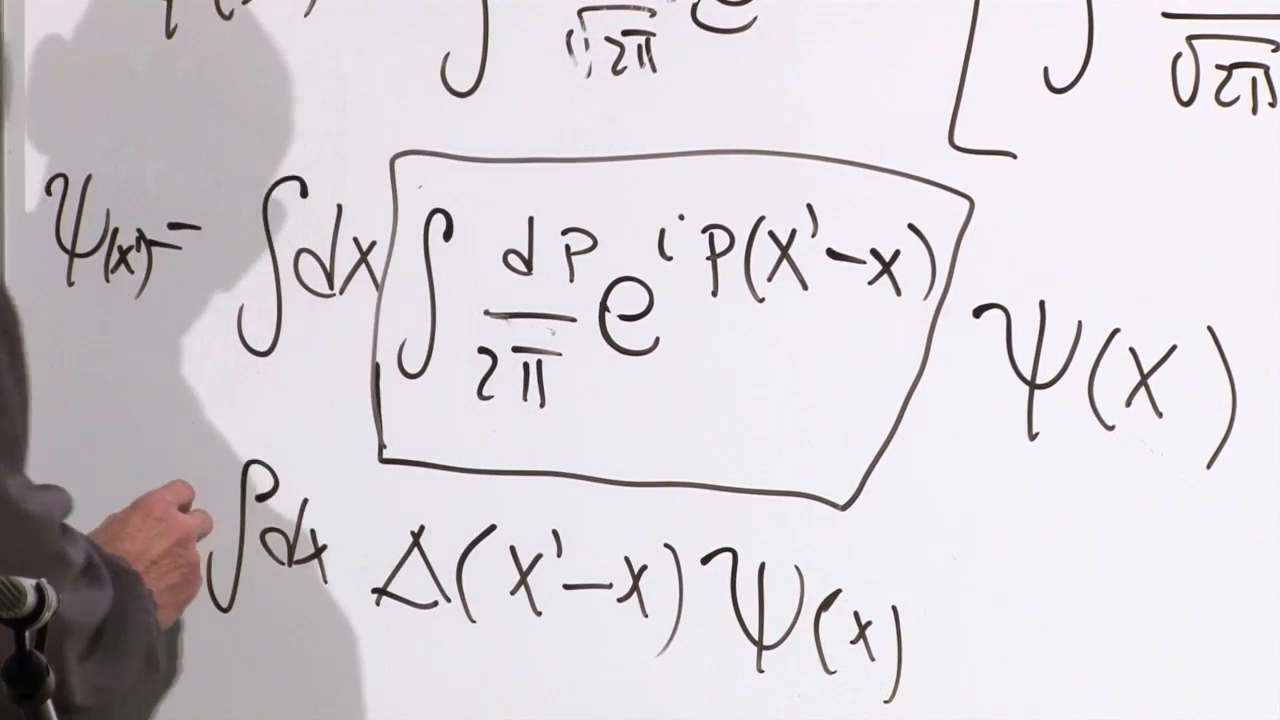
\includegraphics[width=0.88\textwidth]{lecture_09_figure_03.png}
\caption{Tính chất lấy mẫu đặc trưng cho delta Dirac thông qua tác dụng của nó lên mọi hàm thích hợp.}
\lectureframe{00:19:45}
\end{figure}

\begin{classroomqa}
\audiencequestion{Vì sao có thể đưa \(f(x')\) ra ngoài tích phân theo \(x\)?}
\lecturerresponse{Biến tích phân là \(x\). Nhãn \(x'\) được giữ cố định trong phép tích phân đó, nên \(f(x')\) là một hằng số đối với \(x\). Tích phân delta còn lại có diện tích bằng một.}
\end{classroomqa}

Delta không phải là một hàm thông thường xác định theo từng điểm. Đặc biệt, cố gắng bình phương nó dẫn đến một đối tượng kỳ dị hơn delta ban đầu. Cách hiểu an toàn của nó là theo nghĩa phân phối: Phương trình~\eqref{eq:l9-delta-sampling} quy định nó làm gì dưới dấu tích phân.

\subsection{Biểu diễn Fourier của delta}

Thế Phương trình~\eqref{eq:l9-fourier-inverse} vào Phương trình~\eqref{eq:l9-fourier-forward}, đồng thời đổi tên đối số ở vế trái thành \(x'\):
\begin{align}
\psi(x')
&=
\int\frac{dp}{\sqrt{2\pi}}\,
e^{ipx'}
\left[
\int\frac{dx}{\sqrt{2\pi}}\,
\psi(x)e^{-ipx}
\right] \notag\\
&=
\int dx
\left[
\int\frac{dp}{2\pi}
e^{ip(x'-x)}
\right]\psi(x).
\label{eq:l9-fourier-composition}
\end{align}
Biểu thức trong ngoặc vuông phải tái tạo \(\psi(x')\) với mọi \(\psi\) thích hợp. So sánh với tác dụng định nghĩa của delta cho
\begin{equation}
\boxed{
\int_{-\infty}^{\infty}
\frac{dp}{2\pi}\,
e^{ip(x'-x)}
=\delta(x'-x)
}.
\label{eq:l9-delta-fourier-x}
\end{equation}

\begin{figure}[htbp]
\centering
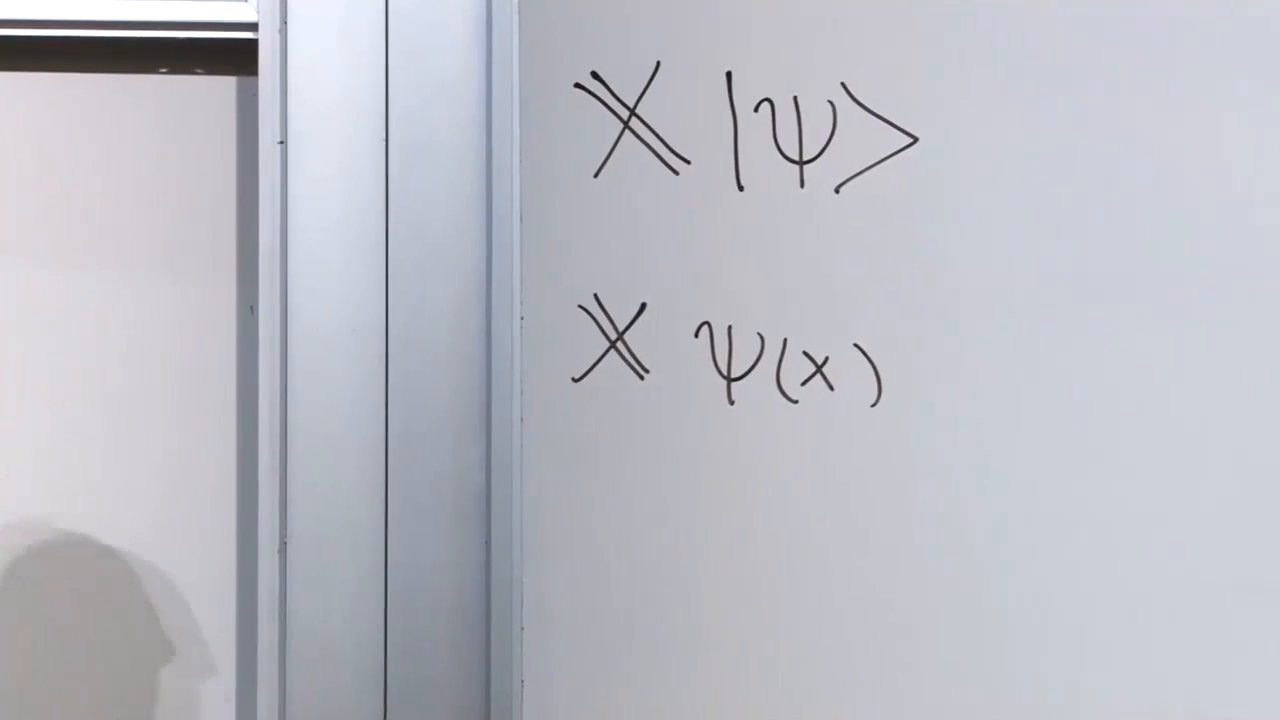
\includegraphics[width=0.88\textwidth]{lecture_09_figure_04.png}
\caption{Hạt nhân Fourier được tách ra trong hợp thành của hai phép biến đổi và được nhận diện, nhờ tính chất lấy mẫu của nó, như một delta Dirac.}
\lectureframe{00:26:23}
\end{figure}

Hoán đổi tên của các biến đối ngẫu cho ta đồng nhất thức đồng hành
\begin{equation}
\boxed{
\int_{-\infty}^{\infty}
\frac{dx}{2\pi}\,
e^{ix(p-p')}
=\delta(p-p')
}.
\label{eq:l9-delta-fourier-p}
\end{equation}
Vì vậy, hàm delta là một chồng chập liên tục của các sóng phẳng.

\begin{classroomqa}
\audiencequestion{Có lúc số mũ được viết là \(x'-x\) và ở chỗ khác lại là \(x-x'\). Việc đổi dấu có làm thay đổi kết quả không?}
\lecturerresponse{Không. Delta là hàm chẵn: \(\delta(u)=\delta(-u)\). Vì thế đảo dấu của hiệu không làm thay đổi phân phối cuối cùng. Hàm mũ trung gian chuyển thành liên hợp phức của nó, nhưng hạt nhân sau khi tích phân vẫn là cùng một delta.}
\end{classroomqa}

Các phép biến đổi này đã lược bỏ một điều kiện về hội tụ. Các tích phân dao động là các phân phối, không phải các tích phân thông thường hội tụ tuyệt đối, và việc đổi thứ tự tích phân đòi hỏi sự cẩn trọng. Một khoảng tuần hoàn hữu hạn cung cấp một bộ điều chuẩn gọn gàng: trước hết dùng các mode Fourier rời rạc và tính trực giao Kronecker, rồi cho khoảng đó tăng không bị chặn. Các đồng nhất thức liên tục ở trên là giới hạn thu được.

\section{Một hạt trên một đường thẳng}

Trong cơ học cổ điển, một điểm trong không gian pha xác định trạng thái:
\begin{equation}
(x,p).
\end{equation}
Cơ học lượng tử đặt ra một câu hỏi đầu tiên khác: cơ sở trực chuẩn nào xác định không gian trạng thái? Với mỗi vị trí thực \(x\), đưa vào một ket riêng suy rộng \(\ket{x}\). Một trạng thái tổng quát có thể được khai triển thành
\begin{equation}
\ket{\Psi}
=
\int_{-\infty}^{\infty}
dx\,\psi(x)\ket{x},
\qquad
\psi(x)=\braket{x}{\Psi}.
\label{eq:l9-position-expansion}
\end{equation}

\begin{figure}[htbp]
\centering
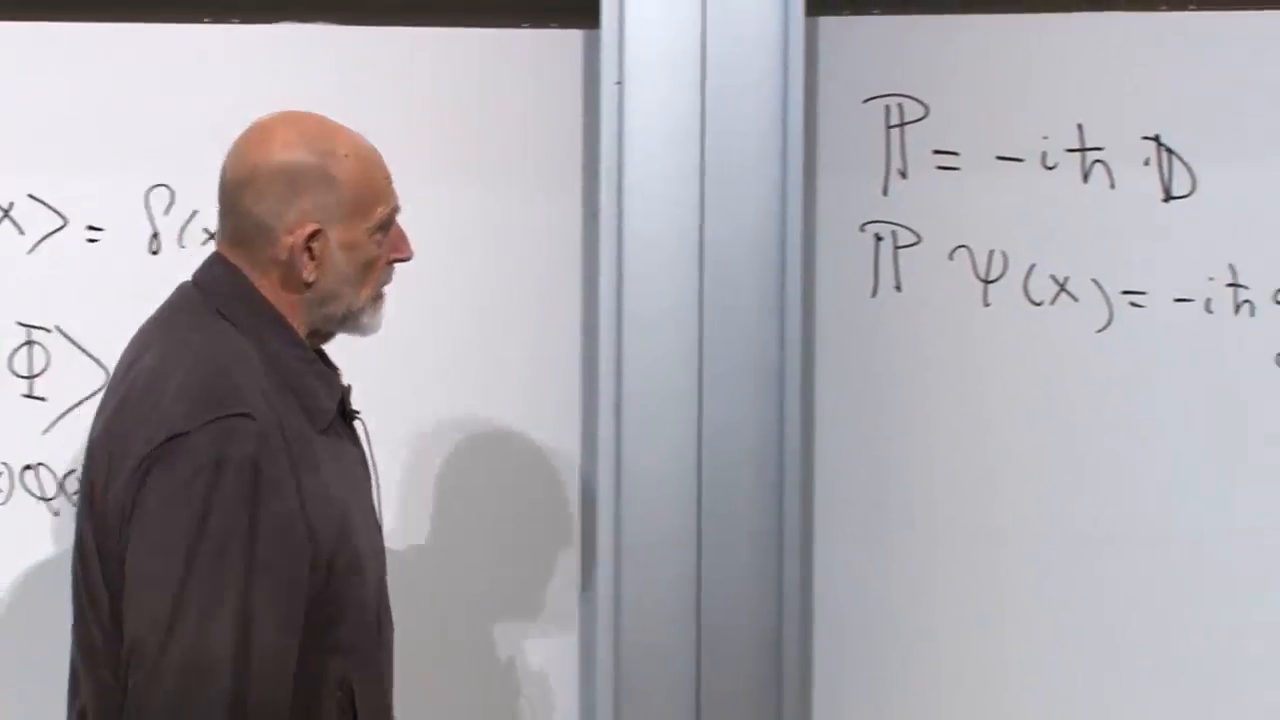
\includegraphics[width=0.88\textwidth]{lecture_09_figure_05.png}
\caption{Một trạng thái tổng quát được khai triển trong cơ sở vị trí liên tục, với hệ số được khôi phục bằng phép chiếu lên \(\ket{x}\).}
\lectureframe{00:35:30}
\end{figure}

Quy tắc Born cho mật độ xác suất
\begin{equation}
\rho(x)=|\psi(x)|^2.
\end{equation}
Xác suất trong một khoảng hữu hạn là
\begin{equation}
P(a<x<b)=\int_a^b|\psi(x)|^2\,dx,
\end{equation}
và một trạng thái vật lý chuẩn hóa thỏa
\begin{equation}
\int_{-\infty}^{\infty}|\psi(x)|^2\,dx=1.
\label{eq:l9-position-normalization}
\end{equation}
Tính trực giao liên tục được biểu diễn bởi
\begin{equation}
\braket{x'}{x}=\delta(x-x').
\label{eq:l9-position-delta}
\end{equation}
Đối với hai trạng thái tùy ý, tích vô hướng trở thành
\begin{equation}
\braket{\Psi}{\Phi}
=
\int_{-\infty}^{\infty}
dx\,\psi^*(x)\phi(x).
\label{eq:l9-position-inner-product}
\end{equation}

\begin{figure}[htbp]
\centering
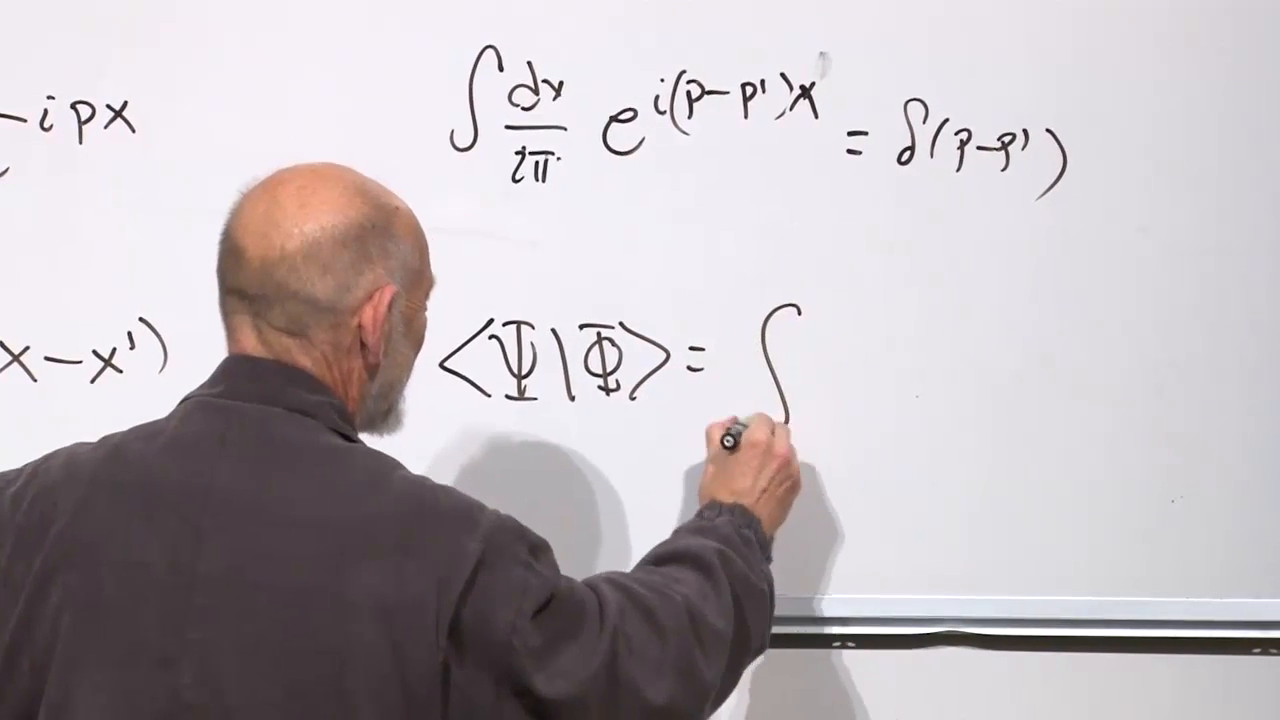
\includegraphics[width=0.88\textwidth]{lecture_09_figure_06.png}
\caption{Chuẩn hóa của cơ sở liên tục và tích vô hướng của hàm sóng được viết trong biểu diễn vị trí.}
\lectureframe{00:41:20}
\end{figure}

\begin{classroomqa}
\audiencequestion{Vì sao chỉ riêng vị trí là đủ? Việc thêm động lượng hay gần như bất kỳ biến nào khác có phải là thừa không?}
\lecturerresponse{Đối với một hạt trong một chiều, toàn bộ hàm \(\psi(x)\) xác định trạng thái, nên một giá trị chính xác đồng thời của \(p\) sẽ là quá nhiều thông tin. Động lượng cung cấp một cơ sở đầy đủ khác chứ không phải một nhãn bổ sung gắn vào mỗi \(\ket{x}\). Trong nhiều chiều hơn, thông tin tương thích có thể được kết hợp: chẳng hạn, \(X\) và \(P_y\) giao hoán và có thể gắn nhãn cho một cơ sở chung. Ràng buộc liên quan đến các cặp không giao hoán, chứ không phải chỉ là số lượng ký hiệu.}
\end{classroomqa}

\begin{classroomqa}
\audiencequestion{Động lượng cũng có thể cung cấp một cơ sở đầy đủ và được khai triển thông qua vị trí chứ?}
\lecturerresponse{Có. Cơ sở động lượng là đầy đủ, và các hệ số của nó liên hệ với các hệ số vị trí bằng phép biến đổi Fourier. Quan hệ đó là cấu trúc trung tâm của bài giảng này.}
\end{classroomqa}

\section{Vị trí trong biểu diễn vị trí}

Một toán tử trừu tượng tác dụng lên các vectơ trạng thái. Khi đã chọn một cơ sở, cùng tác dụng đó trở thành một phép toán cụ thể trên các hàm sóng. Trong biểu diễn vị trí, toán tử vị trí \(X\) tác dụng bằng phép nhân:
\begin{equation}
(X\psi)(x)=x\psi(x).
\label{eq:l9-position-operator}
\end{equation}

Trạng thái định xứ tại \(x_0\) được biểu diễn bởi hàm sóng suy rộng \(\delta(x-x_0)\). Tác dụng \(X\) cho
\begin{align}
X\delta(x-x_0)
&=
x\delta(x-x_0) \notag\\
&=
x_0\delta(x-x_0),
\label{eq:l9-position-eigenfunction}
\end{align}
trong đó đã dùng Phương trình~\eqref{eq:l9-delta-multiplication}. Do đó \(\delta(x-x_0)\) là một hàm riêng của \(X\) với trị riêng \(x_0\).

\begin{figure}[htbp]
\centering
\includegraphics[width=0.88\textwidth]{lecture_09_figure_07.png}
\caption{Phép nhân với \(x\) biến trạng thái định xứ delta thành \(x_0\) lần chính nó, chứng minh rằng nó là một hàm riêng vị trí.}
\lectureframe{00:45:50}
\end{figure}

Cả \(\ket{x_0}\) lẫn biểu diễn bằng hàm delta của nó đều không được chuẩn hóa về 1 theo nghĩa bình phương khả tích thông thường. Ở đây, phép chuẩn hóa là chuẩn hóa delta. Các trạng thái định xứ vật lý là những gói sóng hữu hạn, còn các trạng thái riêng chính xác đóng vai trò như những vectơ cơ sở suy rộng.

\section{Các hàm riêng của xung lượng}

Bài giảng trước đã chỉ ra rằng phép vi phân là phản-Hermite và phép nhân với \(-i\) làm cho nó trở thành Hermite. Khôi phục đơn vị, ta định nghĩa
\begin{equation}
P=-i\hbar\frac{d}{dx},
\qquad
(P\psi)(x)
=
-i\hbar\frac{d\psi}{dx}.
\label{eq:l9-momentum-operator}
\end{equation}
Đây là một đại lượng quan sát được hợp lệ trên một miền xác định thích hợp. Việc đồng nhất nó với xung lượng vật lý sẽ được kiểm tra thông qua phổ, bước sóng và vai trò của nó trong động lực học.

Với một trị riêng xung lượng \(p\), hãy giải
\begin{equation}
P\psi_p=p\psi_p,
\end{equation}
hoặc
\begin{equation}
-i\hbar\frac{d\psi_p}{dx}=p\psi_p.
\end{equation}
Nghiệm là
\begin{equation}
\psi_p(x)=A e^{ipx/\hbar}.
\label{eq:l9-momentum-eigenfunction}
\end{equation}

\begin{figure}[htbp]
\centering
\includegraphics[width=0.88\textwidth]{lecture_09_figure_08.png}
\caption{Biểu diễn trong không gian vị trí của một trạng thái có xung lượng xác định là sóng phẳng \(e^{ipx/\hbar}\).}
\lectureframe{00:51:45}
\end{figure}

Bước sóng \(\lambda\) là độ dời làm cho pha tăng thêm \(2\pi\):
\begin{equation}
\frac{p\lambda}{\hbar}=2\pi,
\qquad
\lambda=\frac{2\pi\hbar}{p}.
\label{eq:l9-de-broglie}
\end{equation}
Vì vậy, xung lượng lớn hơn tương ứng với bước sóng ngắn hơn.

Chuẩn hóa delta xác định hằng số:
\begin{equation}
\psi_p(x)
=
\frac{1}{\sqrt{2\pi\hbar}}e^{ipx/\hbar}.
\label{eq:l9-normalized-momentum-eigenfunction}
\end{equation}
Thật vậy,
\begin{align}
\braket{p'}{p}
&=
\int_{-\infty}^{\infty}
dx\,
\psi_{p'}^*(x)\psi_p(x) \notag\\
&=
\int_{-\infty}^{\infty}
\frac{dx}{2\pi\hbar}
e^{i(p-p')x/\hbar} \notag\\
&=
\delta(p-p').
\label{eq:l9-momentum-normalization}
\end{align}
Sau khi chọn đơn vị sao cho \(\hbar=1\), các công thức này trở thành
\begin{equation}
\psi_p(x)=\frac{1}{\sqrt{2\pi}}e^{ipx},
\qquad
\int\frac{dx}{2\pi}e^{i(p-p')x}
=\delta(p-p').
\end{equation}

\begin{classroomqa}
\audiencequestion{Làm sao có thể tuyên bố rằng tích phân dao động bằng 0 đối với \(p\neq p'\) khi nó không hội tụ theo nghĩa thông thường?}
\lecturerresponse{Bài giảng dùng một lối tắt có kiểm soát. Đặt hệ trong một khoảng hữu hạn với điều kiện biên tuần hoàn. Khi đó các xung lượng được phép tạo thành một tập rời rạc, các hàm mũ trực giao theo nghĩa thông thường, và mọi chuẩn hóa đều hữu hạn. Chỉ sau phép tính ấy mới nên cho khoảng tiến tới vô hạn, biến delta Kronecker thành hàm delta Dirac.}
\end{classroomqa}

\begin{classroomqa}
\audiencequestion{Vấn đề hội tụ tương tự có ảnh hưởng đến phép suy ra hàm delta bằng biến đổi Fourier không?}
\lecturerresponse{Có. Ở đó, việc đổi thứ tự các phép tích phân cũng chỉ là hình thức vì cùng lý do ấy. Cách suy ra trong hộp hữu hạn hoặc ngôn ngữ của các phân bố cung cấp tính chặt chẽ đã bị lược bỏ. Lối tắt này chấp nhận được vì phép tính đã được chính quy hóa có giới hạn liên tục như đã nêu.}
\end{classroomqa}

\section{Biểu diễn xung lượng}

Hai đối tượng này không được nhầm lẫn. Hàm \(\psi_p(x)\) trong Phương trình~\eqref{eq:l9-normalized-momentum-eigenfunction} là biểu diễn trong không gian vị trí của trạng thái riêng cụ thể \(\ket{p}\). Trái lại, hàm sóng trong không gian xung lượng của một trạng thái tùy ý \(\ket{\Psi}\) là
\begin{equation}
\widetilde{\psi}(p)=\braket{p}{\Psi}.
\label{eq:l9-momentum-wavefunction}
\end{equation}
Thế các biểu diễn trong không gian vị trí của \(\bra{p}\) và \(\ket{\Psi}\):
\begin{align}
\widetilde{\psi}(p)
&=
\int_{-\infty}^{\infty}
dx\,
\braket{p}{x}\braket{x}{\Psi} \notag\\
&=
\int_{-\infty}^{\infty}
\frac{dx}{\sqrt{2\pi\hbar}}\,
e^{-ipx/\hbar}\psi(x).
\label{eq:l9-position-to-momentum}
\end{align}
Đây chính xác là biến đổi Fourier. Ngược lại,
\begin{equation}
\psi(x)
=
\int_{-\infty}^{\infty}
\frac{dp}{\sqrt{2\pi\hbar}}\,
\widetilde{\psi}(p)e^{ipx/\hbar}.
\label{eq:l9-momentum-to-position}
\end{equation}

\begin{figure}[htbp]
\centering
\includegraphics[width=0.88\textwidth]{lecture_09_figure_09.png}
\caption{Phép chiếu lên \(\ket{p}\) biến hàm sóng trong không gian vị trí thành biến đổi Fourier của nó, \(\widetilde{\psi}(p)\).}
\lectureframe{01:05:50}
\end{figure}

Mật độ xác suất để đo được xung lượng \(p\) là
\begin{equation}
\widetilde{\rho}(p)
=
|\widetilde{\psi}(p)|^2,
\qquad
\int_{-\infty}^{\infty}
|\widetilde{\psi}(p)|^2\,dp=1.
\end{equation}
Vì thế, một hàm sóng trong không gian vị trí chứa đủ thông tin để dự đoán cả phép đo vị trí lẫn phép đo xung lượng. Để thu được các xác suất xung lượng, hãy biến đổi Fourier \(\psi(x)\) rồi bình phương môđun của kết quả.

Trong biểu diễn xung lượng, vai trò đảo ngược:
\begin{equation}
(P\widetilde{\psi})(p)
=
p\widetilde{\psi}(p),
\qquad
(X\widetilde{\psi})(p)
=
i\hbar\frac{d\widetilde{\psi}}{dp}.
\label{eq:l9-operators-in-p}
\end{equation}
Sự khác biệt về dấu so với \(P=-i\hbar\,d/dx\) xuất phát từ các dấu đối nhau trong cặp Fourier.

\begin{classroomqa}
\audiencequestion{Thời gian có phải là toán tử liên hợp với năng lượng theo cùng cách mà vị trí liên hợp với xung lượng không?}
\lecturerresponse{Thời gian thường được xem như tham số bên ngoài gắn nhãn cho sự tiến hóa của trạng thái, chứ không phải là một toán tử tự liên hợp phổ quát trên không gian Hilbert của hệ. Một đồng hồ vật lý quả thật có các số chỉ quan sát được, và việc cải thiện độ phân giải thời gian của một đồng hồ có hệ quả về năng lượng, nhưng quan hệ thời gian-năng lượng đòi hỏi phải cẩn trọng hơn cặp vị trí-xung lượng và không được phát triển ở đây.}
\end{classroomqa}

\begin{classroomqa}
\audiencequestion{Còn có những cặp liên hợp nào khác?}
\lecturerresponse{Góc và mômen động lượng tương ứng của nó là một ví dụ quan trọng, với những lưu ý toàn cục vì góc là biến tuần hoàn. Trong lý thuyết trường, một trường và xung lượng chính tắc của nó là liên hợp. Nhiệt độ và áp suất là các biến nhiệt động học chứ không phải một cặp lượng tử chính tắc. Nguyên lý tổng quát được cung cấp bởi các biến chính tắc và các giao hoán tử của chúng, chứ không phải bởi một cặp tùy ý nào của các đại lượng đo được.}
\end{classroomqa}

\begin{classroomqa}
\audiencequestion{Trong lý thuyết rời rạc, các toán tử tác dụng lên các ket còn các hàm sóng chỉ đơn thuần liệt kê các hệ số. Điều đó có thay đổi trong lý thuyết liên tục không?}
\lecturerresponse{Không. Một hàm sóng là cột tọa độ của một ket trừu tượng trong một cơ sở đã chọn. Một ma trận tác dụng lên một cột hữu hạn chiều và một toán tử vi phân hay tích phân tác dụng lên một hàm là hai biểu diễn cụ thể của cùng một phép toán trừu tượng. Nhãn liên tục làm thay đổi ký hiệu, chứ không làm thay đổi logic.}
\end{classroomqa}

\subsection{Bất định như một hệ quả Fourier}

Một trạng thái có xung lượng xác định là hoàn toàn không định xứ:
\begin{equation}
|\psi_p(x)|^2=\text{constant}.
\end{equation}
Xung lượng của nó sắc nét, nhưng vị trí của nó trải đều trên toàn bộ trục. Nói chung hơn, một cặp Fourier không thể đồng thời đều hẹp. Việc tập trung \(\widetilde{\psi}(p)\) vào một khoảng xung lượng nhỏ buộc \(\psi(x)\) phải trải ra trên một vùng lớn, và việc định xứ \(\psi(x)\) đòi hỏi một dải xung lượng rộng.

Bài giảng chưa suy ra bất đẳng thức định lượng
\begin{equation}
\Delta X\,\Delta P\geq\frac{\hbar}{2}.
\end{equation}
Điểm cốt yếu hiện tại là về mặt cấu trúc: nguyên lý bất định đã được mã hóa trong hình học tương hỗ của các biến đổi Fourier. Đây là chất tương tự liên tục của việc chuyển giữa các cơ sở spin không tương thích.

\section{Hamiltonian sinh ra sự tiến hóa theo thời gian}

Hamiltonian \(H\) là Hermite, biểu diễn năng lượng, và sinh ra sự tiến hóa đơn nhất theo thời gian. Phương trình Schr\"odinger phụ thuộc thời gian là
\begin{equation}
i\hbar\frac{d}{dt}\ket{\Psi(t)}
=
H\ket{\Psi(t)}.
\label{eq:l9-abstract-schrodinger}
\end{equation}
Trong biểu diễn vị trí,
\begin{equation}
i\hbar\frac{\partial\psi(x,t)}{\partial t}
=
H\psi(x,t),
\label{eq:l9-position-schrodinger}
\end{equation}
trong đó vế phải có nghĩa là biểu diễn trong không gian vị trí đã chọn của Hamiltonian khi nó tác dụng lên hàm.

\subsection{Một Hamiltonian tuyến tính được cố ý chọn cho đơn giản}

Xét
\begin{equation}
H=cP.
\label{eq:l9-linear-hamiltonian}
\end{equation}
Đây không phải là Hamiltonian hạt tự do phi tương đối thông thường. Nó được chọn vì có thể thấy trực tiếp từng bước.

\begin{figure}[htbp]
\centering
\includegraphics[width=0.88\textwidth]{lecture_09_figure_10.png}
\caption{Phương trình Schr\"odinger và Hamiltonian tuyến tính \(H=cP\), được chọn làm ví dụ đơn giản nhất về sự tiến hóa của hạt.}
\lectureframe{01:17:45}
\end{figure}

Dùng \(P=-i\hbar\,\partial_x\),
\begin{align}
i\hbar\frac{\partial\psi}{\partial t}
&=
c\left(-i\hbar\frac{\partial}{\partial x}\right)\psi, \notag\\
\frac{\partial\psi}{\partial t}
&=
-c\frac{\partial\psi}{\partial x},
\end{align}
hoặc
\begin{equation}
\frac{\partial\psi}{\partial t}
+c\frac{\partial\psi}{\partial x}=0.
\label{eq:l9-transport-equation}
\end{equation}

\begin{figure}[htbp]
\centering
\includegraphics[width=0.88\textwidth]{lecture_09_figure_11.png}
\caption{Hamiltonian tuyến tính đưa phương trình Schr\"odinger về phương trình vận chuyển bậc nhất.}
\lectureframe{01:20:05}
\end{figure}

Nghiệm tổng quát là
\begin{equation}
\psi(x,t)=f(x-ct),
\label{eq:l9-rigid-translation}
\end{equation}
đối với mọi biên dạng ban đầu \(f\) chuẩn hóa được. Tại \(t=0\), biên dạng là \(f(x)\). Ở những thời điểm sau đó, mọi đặc trưng đều đã dịch sang phải một đoạn \(ct\). Hàm sóng phức, các phần thực và ảo của nó, và mật độ xác suất của nó đều giữ nguyên hình dạng:
\begin{equation}
|\psi(x,t)|^2=|f(x-ct)|^2.
\end{equation}
Do đó,
\begin{equation}
\expect{X}_t=\expect{X}_0+ct.
\end{equation}

Ký hiệu \(c\) được chọn để gợi đến tốc độ ánh sáng. Mô hình này giống với một kích thích chiral không khối lượng một chiều đơn lẻ: mọi thành phần được phép đều chuyển động theo một hướng với cùng một tốc độ. Nó không phải là một lý thuyết photon hoàn chỉnh. Các phonon một chiều năng lượng thấp với một tốc độ âm thanh cố định tạo nên một phép loại suy khác. Vì \(E=cp\), việc cho phép cả hai dấu của \(p\) cũng cho phép các năng lượng âm, thêm một dấu hiệu nữa cho thấy đây là một mô hình giảng dạy được cố ý giới hạn.

\begin{classroomqa}
\audiencequestion{Liệu \(H=cP\) có mô tả bất kỳ hạt tự do nào nếu \(c\) được thay bằng vận tốc của hạt đó không?}
\lecturerresponse{Không. Một hệ số cố định trong \(H=cP\) nói rằng mọi thành phần xung lượng đều có cùng một vận tốc. Đối với một hạt phi tương đối, vận tốc là \(p/m\), nên nó phụ thuộc vào xung lượng. Viết \(vP\) với \(v=p/m\) không còn tuyến tính theo \(P\) nữa; nó hướng tới một Hamiltonian bậc hai.}
\end{classroomqa}

\begin{classroomqa}
\audiencequestion{Hàm sóng của một electron tự do chuyển động thông thường chẳng phải nên chỉ tịnh tiến nguyên dạng sao?}
\lecturerresponse{Chỉ một quan hệ tán sắc rất đặc biệt mới tạo ra sự tịnh tiến nguyên dạng của mọi biên dạng. Một gói electron tự do thông thường chứa nhiều thành phần xung lượng có pha tiến hóa với những tốc độ khác nhau. Tâm của nó chuyển động, nhưng hình dạng của nó nói chung sẽ dãn rộng.}
\end{classroomqa}

\subsection{So sánh cổ điển}

Đối với Hamiltonian cổ điển \(H=cp\), các phương trình Hamilton cho
\begin{equation}
\dot{x}=\frac{\partial H}{\partial p}=c,
\qquad
\dot{p}=-\frac{\partial H}{\partial x}=0.
\label{eq:l9-linear-hamilton-equations}
\end{equation}

\begin{figure}[htbp]
\centering
\includegraphics[width=0.88\textwidth]{lecture_09_figure_12.png}
\caption{Các phương trình Hamilton cho \(H=cp\): vận tốc không đổi sang phải và xung lượng được bảo toàn.}
\lectureframe{01:25:20}
\end{figure}

Phân bố xác suất lượng tử và giá trị kỳ vọng tương ứng của nó tuân theo cùng chuyển động đơn giản ấy. Sự phù hợp này là lời nhắc cụ thể đầu tiên rằng sự tiến hóa lượng tử được xây dựng từ một Hamiltonian cổ điển phải tái tạo các phương trình cổ điển theo nghĩa thích hợp.

\section{Hạt tự do phi tương đối}

Đối với một hạt thông thường có khối lượng \(m\) và không chịu lực, động năng cổ điển là
\begin{equation}
H=\frac{p^2}{2m}.
\end{equation}
Dạng bậc hai xử lý \(p\) và \(-p\) một cách đối xứng, nên các hạt chuyển động sang trái và sang phải có cùng năng lượng dương. Lượng tử hóa thay \(p\) bằng toán tử \(P\):
\begin{equation}
H=\frac{P^2}{2m}.
\label{eq:l9-free-hamiltonian}
\end{equation}
Thế \(P=-i\hbar\,\partial_x\) vào phương trình Schr\"odinger:
\begin{align}
i\hbar\frac{\partial\psi}{\partial t}
&=
\frac{1}{2m}
\left(-i\hbar\frac{\partial}{\partial x}\right)^2
\psi \notag\\
&=
-\frac{\hbar^2}{2m}
\frac{\partial^2\psi}{\partial x^2}.
\label{eq:l9-free-schrodinger}
\end{align}

\begin{figure}[htbp]
\centering
\includegraphics[width=0.88\textwidth]{lecture_09_figure_13.png}
\caption{Phương trình Schr\"odinger của hạt tự do thu được từ \(H=P^2/(2m)\) và \(P=-i\hbar\,\partial_x\).}
\lectureframe{01:33:50}
\end{figure}

Một thành phần sóng phẳng có xung lượng \(p\) có năng lượng
\begin{equation}
E(p)=\frac{p^2}{2m}.
\end{equation}
Khác với trường hợp tuyến tính \(E=cp\), độ dốc của quan hệ tán sắc này phụ thuộc vào \(p\):
\begin{equation}
v_{\mathrm{group}}
=
\frac{dE}{dp}
=
\frac{p}{m}.
\end{equation}
Vì vậy, các thành phần xung lượng khác nhau của một gói định xứ lan truyền với các vận tốc nhóm khác nhau. Pha tương đối của chúng thay đổi, các thành phần tách ra, và gói sóng dãn rộng. Sự tương phản mang tính quyết định là \(H=cP\) dịch chuyển mọi biên dạng một cách nguyên dạng, còn \(H=P^2/(2m)\) tạo ra chuyển động tán sắc của hạt tự do.

\section{Những điều đã được xác lập}

Phần xen kẽ toán học không tách rời khỏi vật lý. Sóng phẳng và delta Dirac đã xây dựng nên bộ máy cơ sở liên tục. Toán tử vị trí tác dụng bằng phép nhân, toán tử xung lượng tác dụng bằng phép vi phân, và các trạng thái riêng của xung lượng là các sóng phẳng. Phép chiếu một trạng thái tùy ý lên những trạng thái riêng ấy tạo ra biến đổi Fourier của hàm sóng vị trí của nó. Vì thế, vị trí và xung lượng là hai biểu diễn cạnh tranh của cùng một trạng thái, và độ bất định của chúng chính là độ rộng nghịch đảo quen thuộc của một cặp Fourier.

Chính bộ máy biểu diễn ấy sau đó biến một Hamiltonian thành một phương trình vi phân. Một hàm tuyến tính của xung lượng tạo ra sự tịnh tiến nguyên dạng; động năng bậc hai tạo ra phương trình Schr\"odinger của hạt tự do và sự tán sắc. Khóa học đã chuyển từ các nền tảng của phép đo sang cơ học của chuyển động mà không thay đổi ngôn ngữ cốt lõi của mình: trạng thái, cơ sở, các đại lượng quan sát được Hermite, biên độ và sự tiến hóa đơn nhất.
